\documentclass[11pt]{article}
\usepackage[utf8]{inputenc}
\usepackage[T1]{fontenc}
\usepackage[spanish,es-noshorthands]{babel}
\usepackage[margin=2.5cm]{geometry}
\usepackage{amsmath,amssymb}
\usepackage{graphicx}
\usepackage{booktabs}
\usepackage{xcolor}
\usepackage[colorlinks=true,linkcolor=blue,citecolor=blue]{hyperref}
\usepackage{caption}
\usepackage{parskip}
\usepackage[expansion=false]{microtype}
\sloppy

\title{\textbf{Correlación entre las corrientes Monte Carlo\\
de \texttt{analisis\_beta\_optimo.py} y los $\beta$ óptimos reales}}
\author{Walter Quiñonez}
\date{Reporte generado con Claude Code \textperiodcentered\ 5 de septiembre de 2026}

\begin{document}
\maketitle

\begin{quote}\itshape
Este reporte analiza el método que usa \texttt{analisis\_beta\_optimo.py}
para estimar $\beta$ óptimo, y correlaciona la distribución Monte Carlo de
la corriente que ese script construye --- \textbf{antes} y
\textbf{después} de escalarla por los $\beta$ óptimos que efectivamente se
encontraron por grid-search con entrenamiento completo
(\texttt{data\_beta\_grid\_search\_SP/resumen\_por\_INL/resumen\_optimos.csv})---
para explicar por qué esos $\beta$ no la llevan a una escala razonable.
\end{quote}

\tableofcontents

\section{El método de \texttt{analisis\_beta\_optimo.py}}

Para cada una de 3 configuraciones ($p{=}50,a{=}48.83$; $p{=}100,a{=}98.55$;
$p{=}200,a{=}197.99$ --- las tres del grupo INL nominal 1e-2), el script:

\begin{enumerate}
\item Genera las curvas \texttt{pot}, \texttt{dep} con
  \texttt{generar\_curvas\_pot\_dep(...)}.
\item Construye \textbf{\texttt{wij[i,j] = pot[i] - dep[j]} para todas las
  combinaciones $i,j$} (matriz combinatoria completa, tamaño
  $\mathrm{len(pot)}\times\mathrm{len(dep)}$). Esto es distinto de cómo se
  inicializa la red real: en \texttt{G0\_initialization('random', ...)}
  tanto $G^+$ como $G^-$ se sortean, independientemente, del mismo pool
  combinado \{pot\}$\cup$\{dep\} --- acá en cambio se asume que $G^+$ sale
  siempre de la curva \texttt{pot} y $G^-$ siempre de \texttt{dep}.
\item Construye \textbf{\texttt{histograma[i,j] = voltaje\_i} $\cdot$
  \texttt{wij\_j}} (outer product), con \texttt{voltajes =
  np.unique(X\_train)} --- los \textbf{256 niveles de gris distintos}
  presentes en MNIST, cada uno con \textbf{el mismo peso}.
\item Corre un \textbf{Monte Carlo de la corriente}: $I=\sum$ de 784
  términos elegidos al azar (con reposición) de ese pool de productos
  $V{\cdot}W$ --- 1 millón de repeticiones.
\item Con la distribución resultante de $I$, imprime tres candidatos de
  $\beta$ óptimo: $|1/\mathrm{mean}(I)|$,
  $|1/\mathrm{std}(I)+\mathrm{mean}(I)|$ y $1/\mathrm{RMS}(I)$.
\item Finalmente grafica $\beta_r \cdot I$ usando \textbf{los $\beta$
  óptimos ya encontrados en el experimento real}
  (\texttt{betas=[250,350,750]}, que coinciden exactamente con los de
  \texttt{resumen\_optimos.csv} para $p{=}50/100/200$ en INL=1e-2) --- este
  es el paso ``antes/después'' de este reporte.
\end{enumerate}

El propio script trae una nota del autor fechada 18/08: \emph{``no muestra
nada definitivo para relacionar con un beta óptimo''}.

\section{Reproducción y resultados numéricos}

Script nuevo (no modifica \texttt{analisis\_beta\_optimo.py}):
\texttt{reproducir\_analisis\_beta\_optimo.py} --- mismos parámetros y
mismo método; solo vectoriza el Monte Carlo por chunks (en vez de
1.000.000 de llamadas a \texttt{np.random.choice} en un for-loop de
Python) para poder correrlo en segundos.

\begin{table}[htbp]
\centering
\small
\begin{tabular}{@{}rrrrrrrr@{}}
\toprule
$p$ & $\beta$ óptimo & mean($I$) & std($I$) & mean/std & $\beta\cdot$mean($I$) & $\beta\cdot$std($I$) & \%$|\beta I|{>}3$ \\
\midrule
50  & 250 & 0.05211 & 0.00605 & 8.61 & 13.03 & 1.51 & 100\% \\
100 & 350 & 0.05513 & 0.00604 & 9.13 & 19.30 & 2.11 & 100\% \\
200 & 750 & 0.05665 & 0.00603 & 9.39 & 42.49 & 4.52 & 100\% \\
\bottomrule
\end{tabular}
\end{table}

\begin{figure}[htbp]
\centering
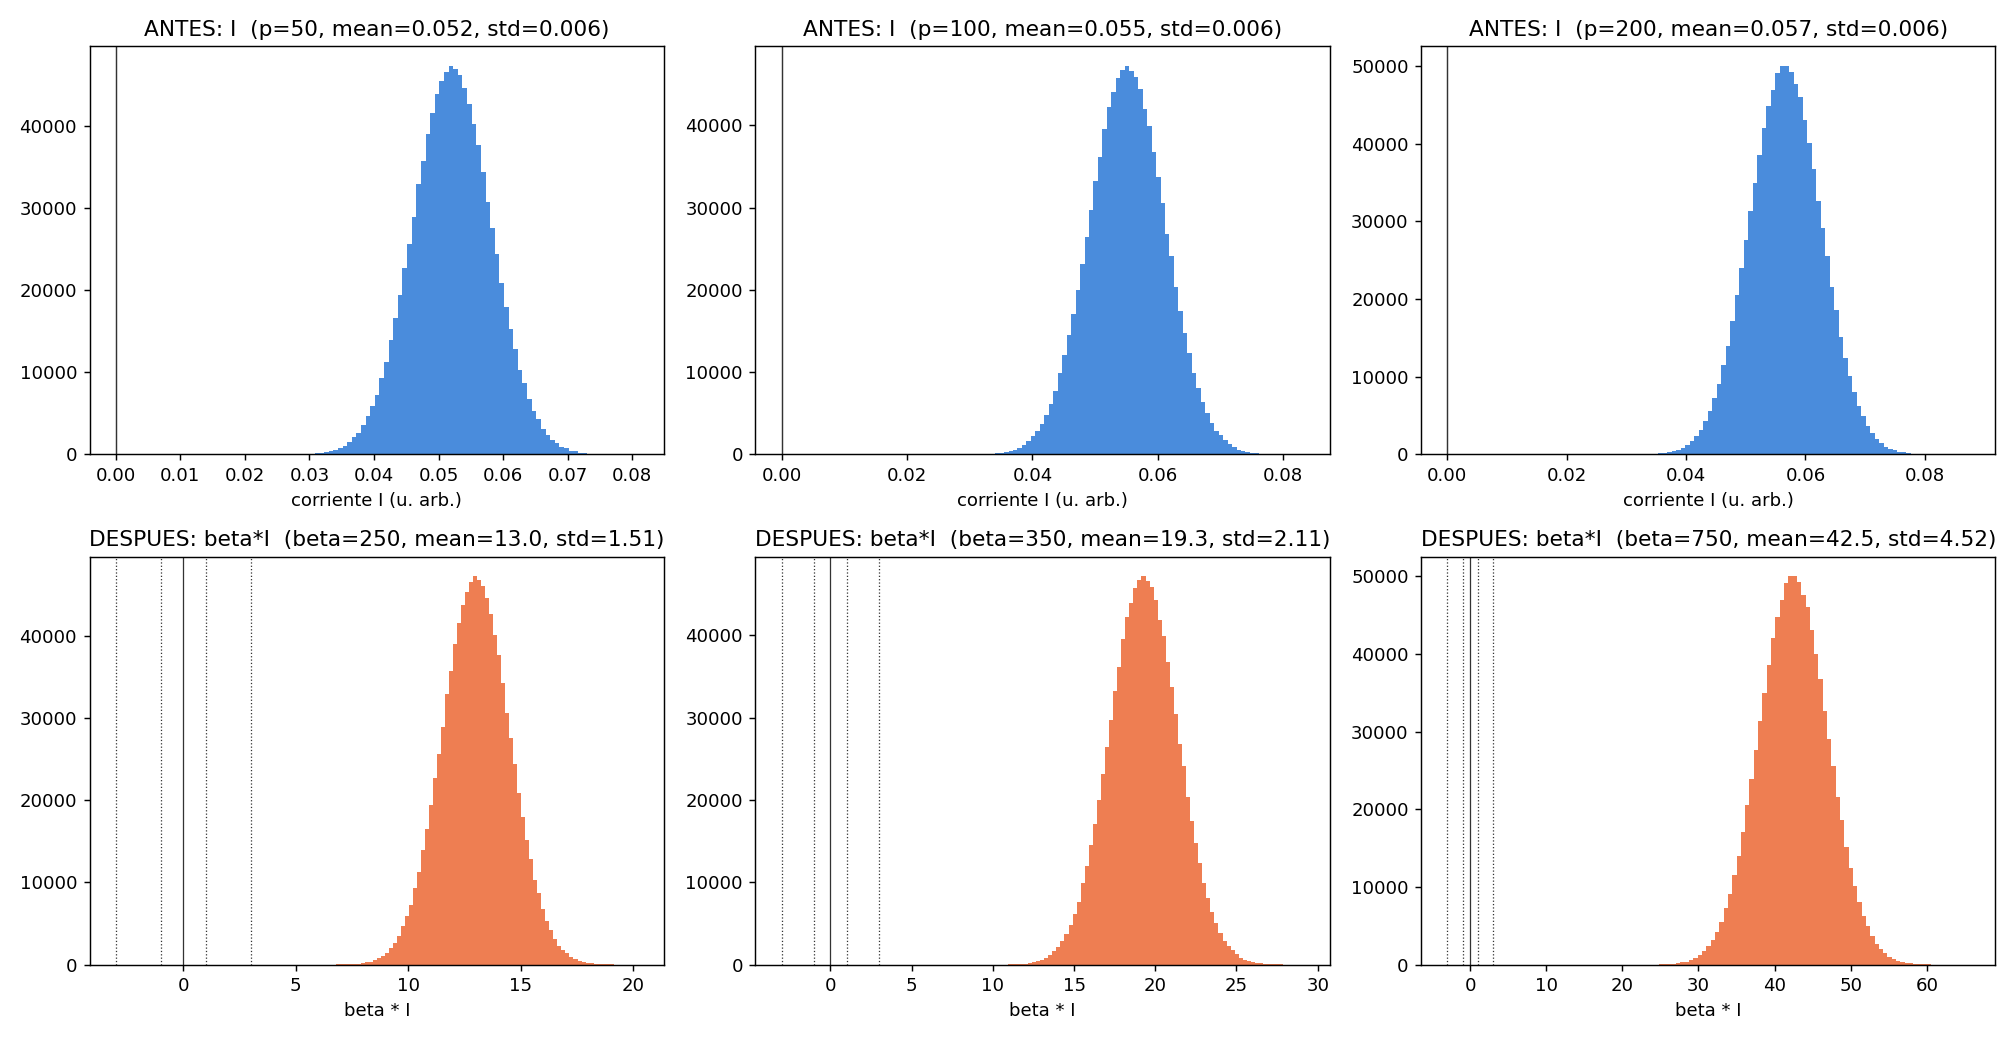
\includegraphics[width=\linewidth]{corrientes_antes_despues_beta.png}
\caption{Arriba: distribución Monte Carlo de $I$ (1M muestras) para cada
curva. Abajo: la misma distribución escalada por el $\beta$ óptimo real de
esa curva, con líneas de referencia en $-3,-1,0,1,3$. Nótese que las líneas
de referencia quedan pegadas al cero, muy lejos del grueso de la
distribución.}
\end{figure}

\section{El hallazgo central}

\textbf{La distribución de $I$ no está centrada en cero.} Su media es
entre 8.6 y 9.4 veces su propio desvío estándar --- es decir, en esta
construcción de Monte Carlo, $I$ se comporta como una constante grande con
una fluctuación chica alrededor, no como una variable de media
aproximadamente nula con dispersión $\sigma_I$ (que es la premisa de la
Ec.~(*) del reporte analítico previo: $\mathbb{E}[I]\approx0$ porque las
curvas son ``diferenciales'').

Al multiplicar por el $\beta$ óptimo real, la distribución se corre y se
ensancha proporcionalmente, pero la razón media/desvío se conserva
(8.6--9.4): el \textbf{100\% de las muestras} caen con $|\beta I|>3$, y la
media escalada crece de 13 a 42 según $p$ --- es decir, la recomendación de
mantener el argumento de la no linealidad en una escala $O(1)$
(LeCun/Prezioso) parece violarse por completo con este $\beta$, y la
violación \textbf{empeora con $p$} --- justo en la misma dirección en que
ya se había visto (en el reporte de validación anterior) que $\beta$
óptimo crecía sin que $\sigma_W$ lo explicara.

\section{Por qué pasa esto (verificado numéricamente)}

$\mathrm{mean}(I) = 784\cdot\mathbb{E}[V]\cdot\mathbb{E}[W]$, y
\textbf{ninguno de los dos factores es cero} aquí:

\begin{table}[htbp]
\centering
\small
\begin{tabular}{@{}lr@{}}
\toprule
Cantidad & Valor \\
\midrule
$\mathbb{E}[V]$ --- voltajes únicos, equipesados (como usa el script) & \textbf{0.500} \\
$\mathbb{E}[V]$ --- \texttt{X\_train} real, todos los píxeles, pesado por frecuencia & \textbf{0.131} \\
$V_{\mathrm{rms}}$ --- voltajes únicos, equipesados & 0.578 \\
$V_{\mathrm{rms}}$ --- \texttt{X\_train} real & 0.335 \\
fracción de píxeles $=0$ en \texttt{X\_train} real & \textbf{80.9\%} \\
\bottomrule
\end{tabular}
\end{table}

\begin{table}[htbp]
\centering
\small
\begin{tabular}{@{}rrrrrr@{}}
\toprule
$p$ & mean(pot) & mean(dep) & $\mathbb{E}[W]$ & $784\cdot\mathbb{E}[V]\cdot\mathbb{E}[W]$ (predicho) & mean($I$) medido \\
\midrule
50  & 6.165e-04 & 4.835e-04 & 1.329e-04 & 0.05210 & 0.05211 \\
100 & 6.203e-04 & 4.797e-04 & 1.406e-04 & 0.05513 & 0.05513 \\
200 & 6.223e-04 & 4.778e-04 & 1.445e-04 & 0.05665 & 0.05665 \\
\bottomrule
\end{tabular}
\caption{La predicción $784\cdot\mathbb{E}[V]\cdot\mathbb{E}[W]$ reproduce
mean($I$) casi exactamente --- la aritmética cierra.}
\end{table}

Dos causas, ambas verificadas, se combinan:
\begin{enumerate}
\item \textbf{$\mathbb{E}[W]=\mathrm{mean(pot)}-\mathrm{mean(dep)}\approx1.3$--$1.4\times10^{-4}\,\mathrm{S}$,
  no es cero.} Las curvas \texttt{pot}/\texttt{dep} generadas (concavidad
  \texttt{pos}/\texttt{neg}) no tienen el mismo promedio global aunque
  cubran el mismo rango $[G_{\min},G_{\max}]$. Esto es una propiedad real
  de la curva, no un artefacto del script.
\item \textbf{$\mathbb{E}[V]=0.5$, muy por encima del promedio real de
  MNIST (0.131).} \texttt{np.unique(X\_train)} toma los 256 niveles de
  gris con el mismo peso, ignorando que el \textbf{81\% de los píxeles
  reales son exactamente 0} (fondo negro). Este sí es un artefacto de
  construcción: un píxel blanco raro pesa en el Monte Carlo igual que el
  fondo negro omnipresente, lo que infla tanto $\mathbb{E}[V]$
  ($\times3.8$) como $V_{\mathrm{rms}}$ ($\times1.7$) respecto de los
  valores reales usados en el reporte de validación anterior.
\end{enumerate}

Multiplicado por los 784 términos de la suma, el sesgo --- minúsculo
término a término --- termina dominando por completo al desvío estándar de
la suma.

\section{Qué dice esto de los 3 candidatos de $\beta$ que imprime el script}

\begin{table}[htbp]
\centering
\small
\begin{tabular}{@{}lrrrl@{}}
\toprule
Candidato & $p=50$ & $p=100$ & $p=200$ & vs.\ $\beta$ óptimo real \\
\midrule
$1/\mathrm{mean}(I)$ & 19.19 & 18.14 & 17.65 & 13$\times$--43$\times$ más chico \\
$|1/\mathrm{std}(I)+\mathrm{mean}(I)|$ & 165.24 & 165.66 & 165.81 & 1.5$\times$--4.5$\times$ más chico, casi constante \\
$1/\mathrm{RMS}(I)$ & 19.06 & 18.03 & 17.55 & 13$\times$--43$\times$ más chico \\
\bottomrule
\end{tabular}
\end{table}

Los tres subestiman fuertemente al $\beta$ óptimo real (250--750),
consistente con la Sección 4: al estar construidos sobre una $I$ con media
y dispersión infladas por el sesgo de $\mathbb{E}[V]$ y $\mathbb{E}[W]$,
sus recíprocos quedan chicos.

\textbf{Nota sobre $|1/\mathrm{std}(I)+\mathrm{mean}(I)|$:} esta expresión
sale de \texttt{np.abs(1/(np.std(corrientes)) + np.mean(corrientes))} ---
es decir, suma $1/\mathrm{std}$ (unidades de 1/corriente) con
$\mathrm{mean}$ (unidades de corriente), lo cual no es dimensionalmente
consistente. Su casi-constancia frente a $p$ (165.2, 165.7, 165.8) se
explica porque $\mathrm{std}(I)$ apenas cambia entre las tres curvas
(0.00603--0.00605) mientras que $\mathrm{mean}(I)$ es demasiado chico
frente a $1/\mathrm{std}(I)\approx166$ como para moverlo. Todo indica un
error de paréntesis (quizás se buscaba $1/(\mathrm{std}(I)+\mathrm{mean}(I))$),
no una fórmula deliberada.

\section{Conclusión}

El método de \texttt{analisis\_beta\_optimo.py} no es un buen predictor de
$\beta$ óptimo, y ahora se puede explicar con precisión por qué: no falla
por falta de señal en el problema, sino porque su Monte Carlo respira una
distribución de voltajes de entrada (\texttt{np.unique(X\_train)},
equipesada) que \textbf{no representa las imágenes reales} (81\% de fondo
negro) ni la asimetría real entre las curvas \texttt{pot}/\texttt{dep}. El
resultado es una $I$ cuya media domina a su propia dispersión por casi un
orden de magnitud, así que ningún múltiplo razonable de
$1/\mathrm{mean}(I)$, $1/\mathrm{std}(I)$ o $1/\mathrm{RMS}(I)$ puede
coincidir con el $\beta$ óptimo real (que sí sitúa la red en su mejor
accuracy empírica).

Esto es consistente con --- y ayuda a entender retroactivamente --- por
qué el proyecto pasó de este script exploratorio a la fórmula analítica
basada en $\sigma_W$ real (vía \texttt{G0\_initialization}, que sí sortea
$G^+$ y $G^-$ del mismo pool combinado) y $V_{\mathrm{rms}}$ calculado
directamente sobre \texttt{X\_train\_mnist.npy} completo
(\texttt{papers/Reporte\_beta\_optimo\_analitico.pdf}, validada con datos
reales en \texttt{validacion\_formula\_beta\_optimo/}): esa fórmula evita
ambos sesgos identificados acá.

\section{Registro de códigos usados}

\begin{itemize}
\item \texttt{analisis\_beta\_optimo.py} --- Archivo analizado (no
  modificado); fuente de los parámetros, la construcción de
  \texttt{wij}/\texttt{histograma}, el Monte Carlo de $I$ y los 3
  candidatos de $\beta$ descriptos en la Sección 1.
\item \textbf{\texttt{reproducir\_analisis\_beta\_optimo.py}} --- Único
  script nuevo. Reproduce el mismo método (vectorizado) para poder
  extraer números y figuras; genera
  \texttt{corrientes\_antes\_despues\_beta.csv},
  \texttt{diagnostico\_voltajes.csv} y
  \texttt{corrientes\_antes\_despues\_beta.png}.
\item \texttt{MemCrossbarClass\_beta\_por\_capa.py}
  $\to$ \texttt{generar\_curvas\_pot\_dep()} --- Genera las curvas
  \texttt{pot}/\texttt{dep} reales de las 3 configuraciones (sin
  modificar).
\item \texttt{data\_beta\_grid\_search\_SP/resumen\_por\_INL/resumen\_optimos.csv}
  --- Fuente de los $\beta$ óptimos reales (250, 350, 750) usados en el
  paso ``después''.
\item \texttt{X\_train\_mnist.npy} --- Dataset real, usado tanto por el
  método original (\texttt{np.unique}) como para el diagnóstico de la
  Sección 4 (media/RMS reales, pesados por frecuencia).
\end{itemize}

Archivos generados por este reporte (todos en
\texttt{analisis\_corrientes\_beta\_optimo/}):
\texttt{reproducir\_analisis\_beta\_optimo.py},
\texttt{corrientes\_antes\_despues\_beta.csv},
\texttt{diagnostico\_voltajes.csv},
\texttt{corrientes\_antes\_despues\_beta.png},
\texttt{reporte\_correlacion\_corrientes\_beta.tex} y este PDF.

\end{document}
